\chapter{Creating New Boards}

First get the source code and compile as described in \hyperlink{def:isource}{Install from source}.

\section{Creating a New Board}

The first step is get the schematic and all information about the board hardware.
The second step is the creation of four files in PICSimLab dir (consider replace the 'x' of board\_x for a number or name in your case):
\begin{itemize}
\item Board Picture (share/boards/x/board.svg) or (share/boards/x/board.png);
\item Board map (share/boards/x/board.map);
\item Board header (src/boards/board\_x.h);
\item Board C++ code (src/boards/board\_x.cc);
\end{itemize}

The third and last step is recompiling PICSimLab with new board support.

\subsection{Board Hardware and Schematic}

For this tutorial, the board created have the hardware shown in diagram below:
\begin{figure}[H]
\center
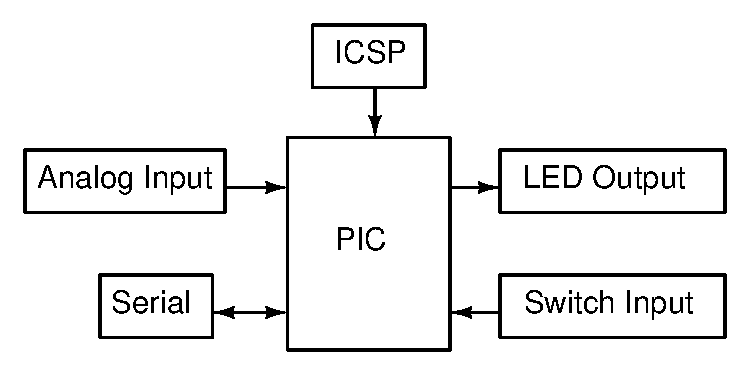
\includegraphics[width=0.7\textwidth]{img/hb/blocks.eps} 
\end{figure} 

The schematic for the tutorial board made in \href{http://kicad-pcb.org/}{Kicad}.
\begin{figure}[H]
\center
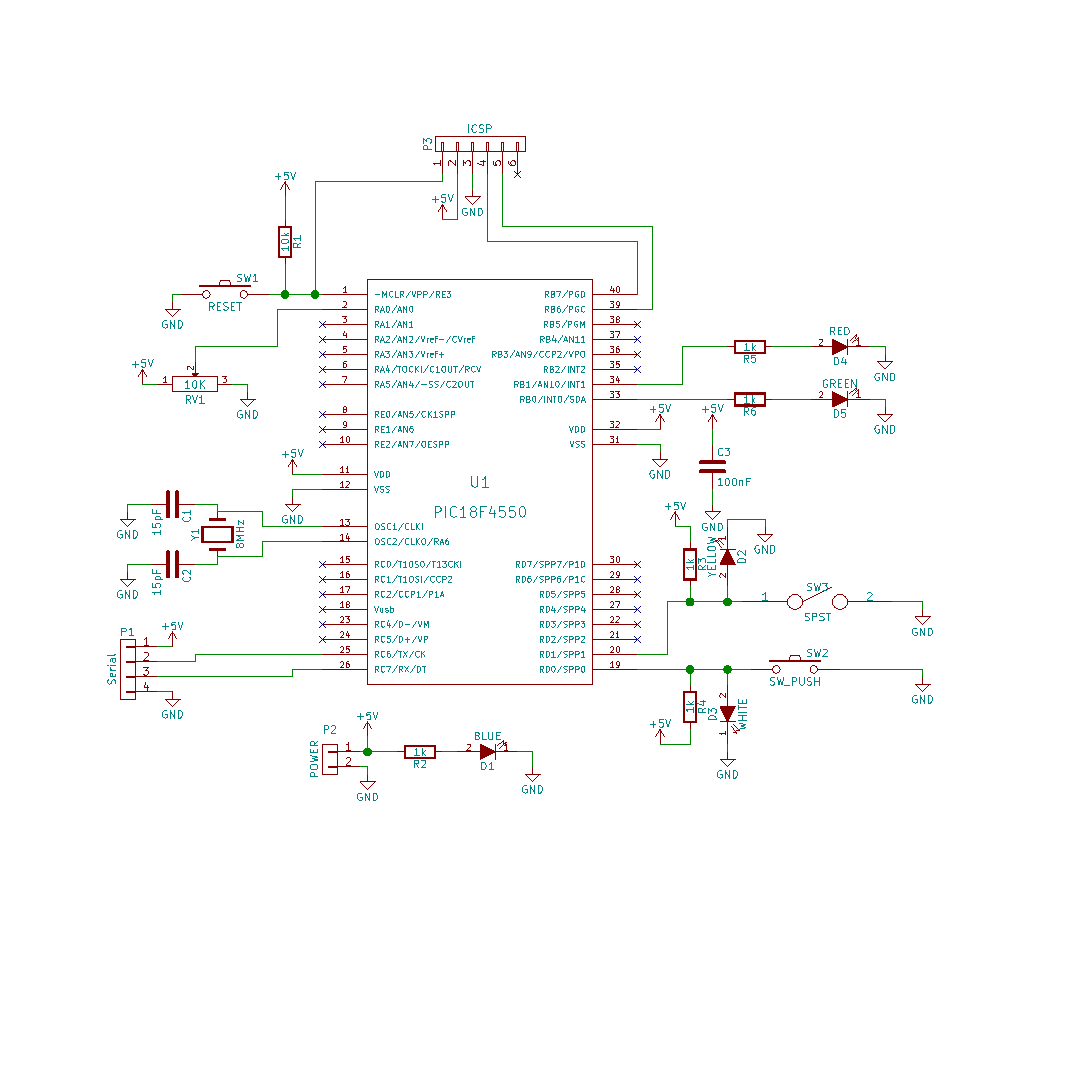
\includegraphics[width=0.99\textwidth]{board_x/board_x.eps} 
\end{figure} 

\pagebreak
And the PCB layout was made in \href{http://kicad-pcb.org/}{Kicad} too. The PCB is not necessary if you have a real board.

\begin{figure}[H]
\center
\includegraphics[width=0.9\textwidth, angle=0]{board_x/board_x_pcb.eps} 
\end{figure} 

\pagebreak
\subsection{Board Picture}

The PNG board picture was taken from \href{http://kicad-pcb.org/}{Kicad} 3D viewer.
The picture image is saved as ``share/board/x/board.png''.

\begin{figure}[H]
\center
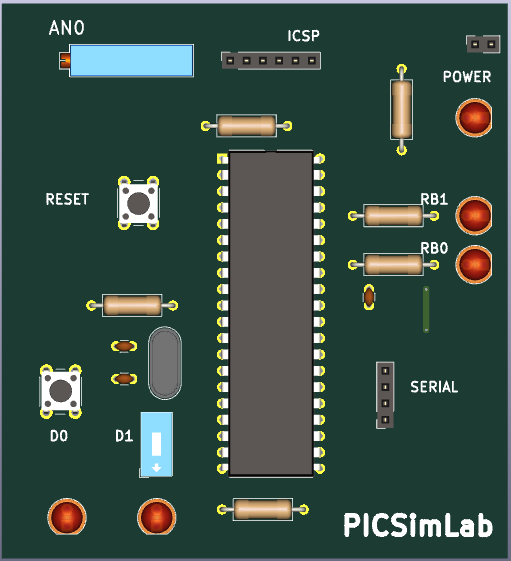
\includegraphics[width=0.8\textwidth]{files/share/board.png} 
\end{figure} 

It is also possible to use images in SVG format for better viewing quality. \href{https://github.com/yaqwsx/PcbDraw}{PCBDraw} can be used to convert a Kicad PCB project to 
an SVG image. 

\begin{figure}[H]
\center
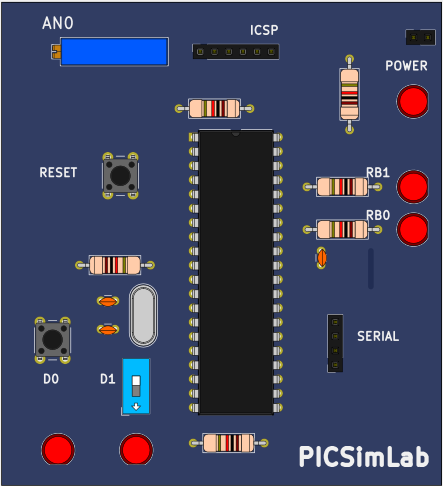
\includegraphics[width=0.8\textwidth]{files/share/board_svg.png} 
\end{figure} 

\pagebreak
\subsection{Picture map}
The PICSimLab use one picture image map for inputs and outputs. 

The inputs are the areas in board picture which user can interact (by mouse click) and 
start with letters ``I\_''. 

The output are the areas in board picture to be redraw according simulator status and start with
letters ``O\_''. 

The bidirectional areas in board picture which user can interact and need to be redraw according simulator status 
are started with letter ``B\_''. 

The picture map used for PICSimLab are normal HTML image-map. They can be made by hand or using any software which 
can handle image maps. The original PICSimLab maps are made using \href{http://www.gimp.org/}{Gimp image editor}.     

To start, in the GIMP, use the Filters->Web->Image Map to open image map editor window.
\begin{figure}[H]
\center
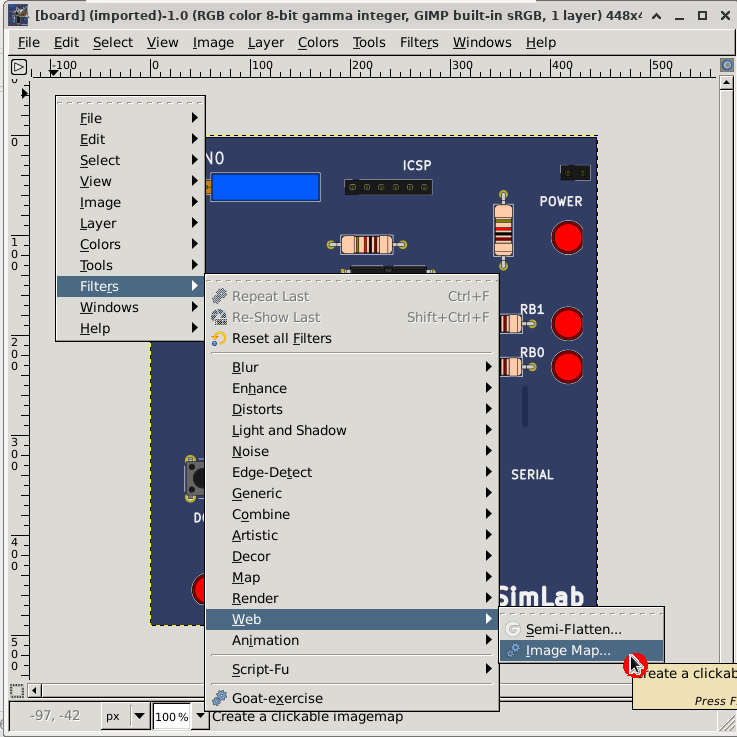
\includegraphics[width=0.99\textwidth]{img/hb/gimp01.png} 
\end{figure} 

\pagebreak
Then select rectangle or circle map on toolbar.
\begin{figure}[H]
\center
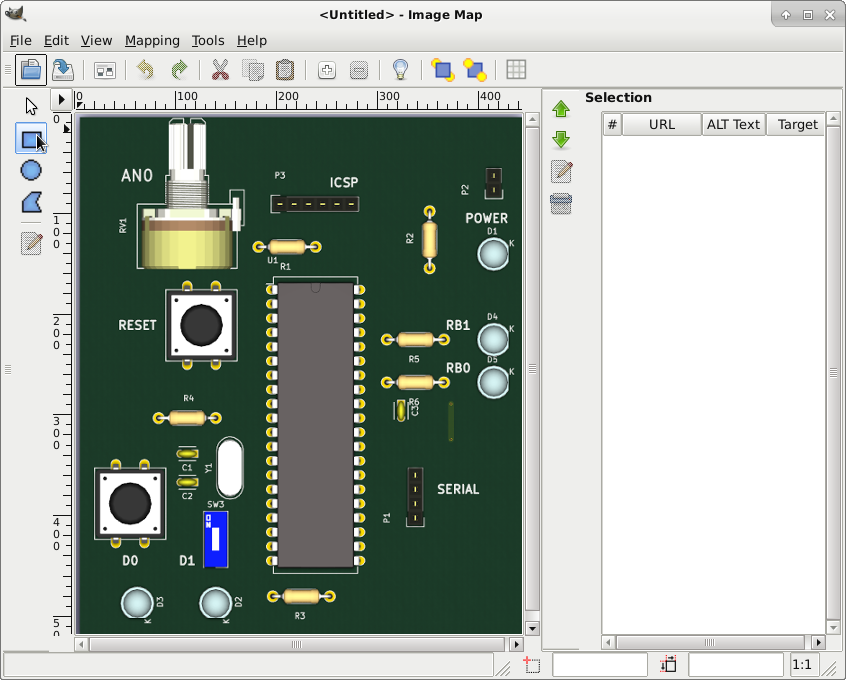
\includegraphics[width=0.8\textwidth]{img/hb/gimp02.png} 
\end{figure} 

And mark the area in picture.
\begin{figure}[H]
\center
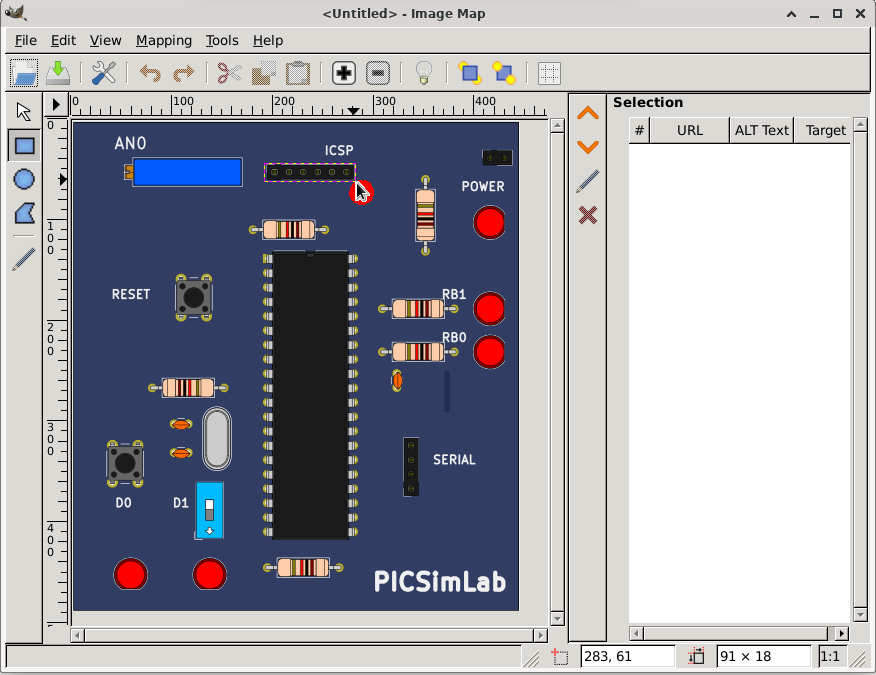
\includegraphics[width=0.8\textwidth]{img/hb/gimp03.png} 
\end{figure} 

\pagebreak
After area is select, in the settings windows select the link type for ``Other''. 
\begin{figure}[H]
\center
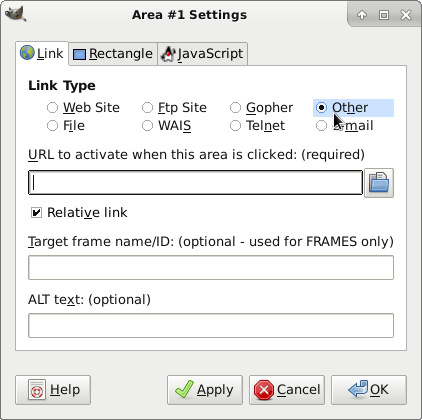
\includegraphics[width=0.7\textwidth]{img/hb/gimp04.png} 
\end{figure} 

And write the name of area. The name must describe the area function on the board 
and follow the \hyperlink{def:map}{Picture Map Reference}.

\begin{figure}[H]
\center
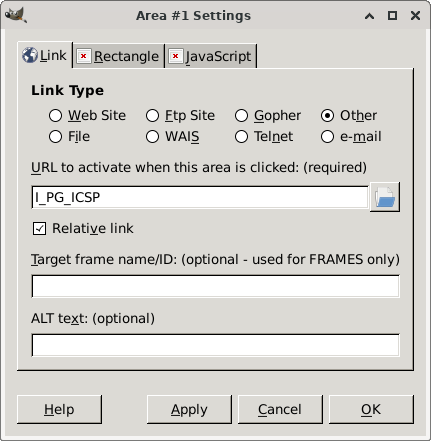
\includegraphics[width=0.7\textwidth]{img/hb/gimp05.png} 
\end{figure} 


\subsubsection{Board map}

For this tutorial board, twelve areas are marked:
\begin{itemize}
\item I\_PG\_ICSP - where user click to load hexfile.
\item I\_SW\_PWR - where user click to turn on/off the board.
\item B\_SW\_D1 - Switch connected in RD1.
\item B\_PO\_1 - Potentiometer connected to RA0.
\item B\_PB\_RST - Button to reset board.
\item B\_PB\_D0 - Button connected in RD0. 
\item O\_LD\_LD0 - draw LED connected in push button D0.
\item O\_LD\_LD1 - draw LED connected in switch D1.
\item O\_LD\_LPWR - draw power LED indicator.
\item O\_LD\_RB1  - draw LED connected in RB1.
\item O\_LD\_RB0  - draw LED connected in RB0.
\item O\_IC\_CPU  - draw microcontroller name.
\end{itemize}


\begin{figure}[H]
\center
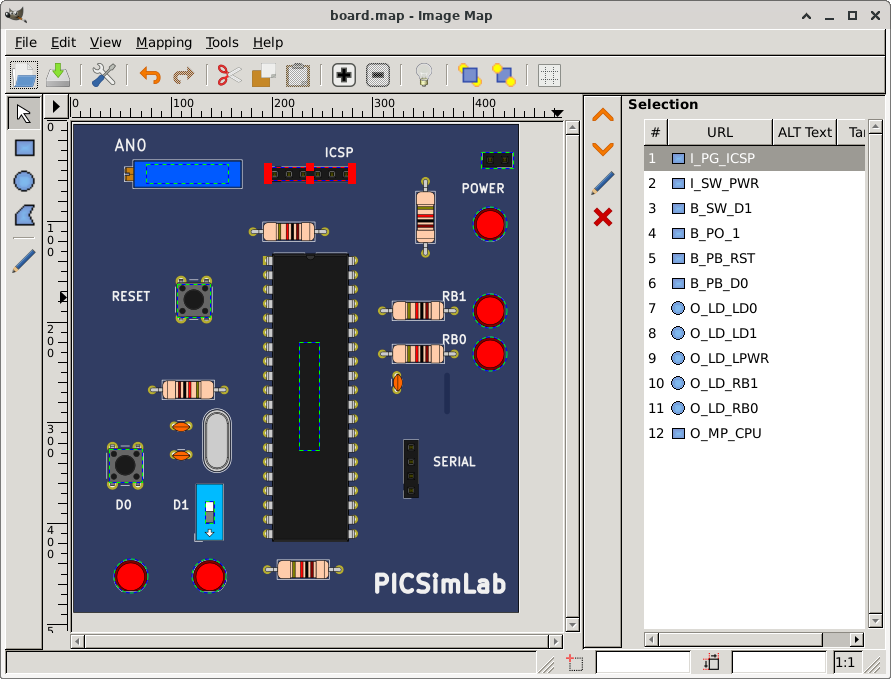
\includegraphics[width=0.7\textwidth]{img/hb/gimp06.png} 
\end{figure} 


Board map generated by Gimp image map editor and saved as ``share/boards/X/board.map''.
\inputminted[baselinestretch=1.2,fontsize=\footnotesize,linenos]{html}{files/share/board.map}

The kicad project files can be download from github \href{https://github.com/lcgamboa/picsimlab_docs/tree/main/kicad/board_x}{PICSimLab repository}. 

\subsection{Board code}

The header file and c++ code file with comments are listed in the next two subsections. This files control the behavior of board in simulator.

\subsubsection{board\_x.h}

\href{https://github.com/lcgamboa/picsimlab/blob/master/src/boards/board_x.h}{ board\_x.h online file}.

\href{https://lcgamboa.github.io/picsimlab_docs/devel/html/index.html#binc}{ board\_x.h online doxygen version}.


\inputminted[baselinestretch=1.2,fontsize=\footnotesize,linenos]{c++}{files/board_x.h}

\pagebreak
\subsubsection{board\_x.cc}

\href{https://github.com/lcgamboa/picsimlab/blob/master/src/boards/board_x.cc}{ board\_x.cc online file}.

\href{https://lcgamboa.github.io/picsimlab_docs/devel/html/index.html#bcode}{ board\_x.cc online doxygen version}.

\inputminted[baselinestretch=1.2,fontsize=\footnotesize,linenos]{c++}{files/board_x.cc}


\subsection{Integration with PICsimLab}

To integration of the new board in PICSimLab, are necessary edit one file.

The file is Makefile.Common. The only change to be made is include object \textbf{boards/board\_board\_x.o} in 
 objects list. They can be added in variable OBJS or OBJS\_EXP (used only in experimental version).

After change the Makefile.Common and include the five files created for new board, the PICSimLab can be recompiled,
as described in \hyperlink{def:isource}{Install from source}.


\subsection{Final Result}

The PICSimLab board created for this tutorial are shown in the figure below.
\begin{figure}[H]
\center
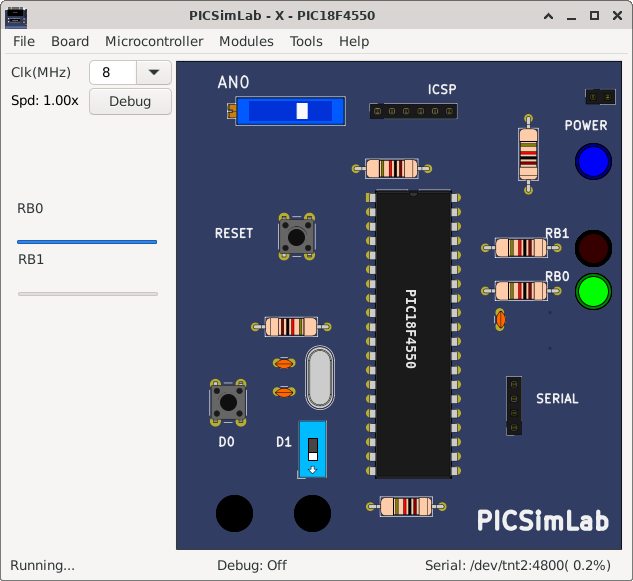
\includegraphics[width=0.9\textwidth]{img/hb/final.png} 
\end{figure} 

The sample program below can be used to test new board, this code is write for XC8 compiler:
\inputminted[baselinestretch=1.2,fontsize=\footnotesize,linenos]{c}{sample/board_x.c}

